\documentclass[aspectratio=169]{beamer}

%%% Работа с русским языком
\usepackage{cmap}					% поиск в PDF
\usepackage{mathtext} 				% русские буквы в формулах
\usepackage[T2A]{fontenc}			% кодировка
\usepackage[utf8]{inputenc}			% кодировка исходного текста
\usepackage[english,russian]{babel}	% локализация и переносы
\usepackage{indentfirst}
\frenchspacing

%%% Дополнительная работа с математикой
\usepackage{amsmath,amsfonts,amssymb,amsthm,mathtools}  % AMS

%%% Текст в колонки
\usepackage{multicol}

%%% Системы уравнений
\usepackage{cases}

%%% Таблицы
\usepackage{array}

%%% Картинки
\usepackage{graphicx}
\usepackage{float}

%%% Список литературы
\usepackage[sorting=none]{biblatex}
\renewbibmacro{in:}{\ifentrytype{article}
    {}
    {\bibstring{in}\printunit{\intitlepunct}}
}
\addbibresource{references.bib}

%%% Гиперссылки
\usepackage{hyperref}

%%% Перенос знаков в формулах (по Львовскому)
\newcommand*{\hm}[1]{#1\nobreak\discretionary{}
{\hbox{$\mathsurround=0pt #1$}}{}}


%%% Свои команды

\newcommand{\vect}[1]{\textbf{#1}}
\newcommand{\vx}{{\vect{x}}}
\newcommand{\vn}{{\vect{n}}}

\newcommand{\half}{\cfrac{1}{2}}

\newcommand{\partt}[1]{\cfrac{\partial #1}{\partial t}}
\newcommand{\partx}[1]{\cfrac{\partial #1}{\partial x}}
\newcommand{\partxx}[1]{\cfrac{\partial^2 #1}{\partial x^2}}
\newcommand{\partvn}[1]{\cfrac{\partial #1}{\partial \vn}}

\newcommand{\partflt}[1]{\partial #1 / \partial t}
\newcommand{\partflx}[1]{\partial #1 / \partial x}
\newcommand{\partflxx}[1]{\partial^2 #1 / \partial x^2}
\newcommand{\partflvn}[1]{\partial #1 / \partial \vn}

\newcommand{\gradsq}[1]{(\nabla #1, \nabla #1)}

\newcommand{\difftau}[1]{\cfrac{{#1}_j^{k + 1} - {#1}_j^k}{\tau}}
\newcommand{\diffhh}[1]{\cfrac{{#1}_{j + 1}^k - 2 {#1}_j^k + {#1}_{j - 1}^k}{h^2}}

\newcommand{\Natural}{{\mathbb{N}}}
\newcommand{\Real}{{\mathbb{R}}}
\newcommand{\bigO}{{\mathcal{O}}}
\newcommand{\clOmega}{{\overline{\Omega}}}

\newcommand{\norm}[1]{\| \, #1 \, \|}
\newcommand{\enorm}{{\| \cdot \|}}

\newcommand{\unitm}{{\text{м}}}
\newcommand{\units}{{\text{с}}}
\newcommand{\unitJ}{{\text{Дж}}}
\newcommand{\unitC}{{\text{Кл}}}
\newcommand{\unitV}{{\text{В}}}
\newcommand{\unitF}{{\text{Ф}}}

\newcommand{\nologo}{\setbeamertemplate{logo}{}}


%%% Свои операторы
\DeclareMathOperator{\Div}{{div}}
\DeclareMathOperator{\Const}{{const}}

%%% Цвета
\definecolor{green}{RGB}{0,200,0}
\definecolor{red}{RGB}{200,0,0}

%%% Тема оформления
\usetheme{Madrid}


%%% Титульный лист
\title[Адаптация шага по времени]{Сравнение методов адаптации шага по времени \\ в модели типа диффузной границы, \\ включающей уравнение Аллена–Кана}
\author[]{
	Зипунова Е. В.\textsuperscript{1}, \underline{Пономарев А. С.}\textsuperscript{1,2}, Савенков Е. Б.\textsuperscript{1}
}
\institute[ИПМ, МФТИ]{
	\textsuperscript{1}ИПМ им. М. В. Келдыша РАН \\
	\textsuperscript{2}МФТИ (НИУ)
}
\date[Новые горизонты]{
	Новые горизонты прикладной математики \\[1mm]
	18.04.2025
}
\logo{
\includegraphics[height=0.8cm]{../figures/labels.jpg}}


\begin{document}

\AtBeginSection[]{
	\begin{frame}{Содержание}
	\Large
	\tableofcontents[currentsection]
	\end{frame}
}

\begin{frame}
\titlepage
\end{frame}

\begin{frame}{Содержание}
\Large
\tableofcontents
\end{frame}


%!TEX root = ../main.tex

\section{Введение}

Электрический пробой~-- это явление резкого возрастания тока в диэлектрике при приложении электрического напряжения выше некоторого критического значения. Механизм разрушения диэлектрика под действием электрического поля сложен и многообразен: оно может иметь различные причины, характер развития, сопутствующие физические процессы \cite{vorobiev_dielectric_physics}.

Среди многообразия математических моделей, созданных для описания развития канала электрического пробоя, выделим предложенную в работе \cite{pitike_dielectric_breakdown} модель типа диффузной границы.

В настоящее время модели типа диффузной границы составляют целый класс подходов для решения задач в различных областях науки и техники. В частности, описанная в работе \cite{pitike_dielectric_breakdown} модель построена как формальное обобщение ранее известных моделей типа диффузной границы, применяемых в теории трещин.

Исследование и дальнейшее развитие упомянутой модели можно найти в работах \cite{zipunova_higher_codimension, zipunova_conservative, zipunova_thermomechanical, ponomarev_stability}. Основные положения метода диффузной границы в применении к моделированию развития канала электрического пробоя перечислены в работе \cite{ponomarev_stability}.

Модели типа диффузной границы используются для описания систем, в которых вещество может находиться в нескольких различных состояниях~-- фазах,~-- причем вещество в одной и той же фазе образует некоторые однородные области. В моделях типа диффузной границы распределение фаз вещества задается гладкой функцией $\phi$~-- фазовым полем,~-- которая в каждой области однородности близка к постоянной. Характерная толщина разделяющего слоя (<<диффузной границы>>) и, соответственно, скорость изменения~$\phi$ при переходе от одной фазы к другой определяется параметрами модели.

В работе \cite{zipunova_higher_codimension} проводится исследование свойства упомянутой модели развития канала электрического пробоя, которое можно назвать коразмерностью <<включений>>. Для задач теории трещин естественным будет двумерное включение (плоская трещина) в трехмерной среде вещества~-- в таком случае говорят, что коразмерность объекта равна 1. Обратим внимание, что, хотя исследуемая модель, как было сказано, получена на основе моделей из теории трещин, для нее характерным будет одномерное включение (канал пробоя), то есть имеющее коразмерность 2. В работе \cite{zipunova_higher_codimension} указано, что это может привести к нетривиальным последствиям, и предложено определенное обобщение исходной модели, которое предположительно делает ее более адекватной.

Суть обобщения состоит в формальном добавлении в уравнения модели двух слагаемых высших порядков с некоторыми коэффициентами. Целью настоящей работы является численная проверка поведения модели при различных значениях коэффициентов. Для этого ищется стационарное распределение фазового поля $\phi$ в нескольких характеристических случаях. Построение разностной схемы для задачи несет определенные сложности, связанные с необходимостью задать граничные условия на множествах коразмерности~2 и~3 в трехмерном пространстве. Предполагается, что точках этих множеств функция фазового поля $\phi$ имеет особенность.

Авторами применена модификация метода конечных объемов. Для части конфигураций обобщенной модели она позволила составить разнотную схему. Создана компьютерная программа, реализующая схему; проделаны расчеты, их результаты приведены в виде графиков. Для остальных конфигураций модели в процессе применения метода возникли фундаментальные проблемы, что позволяет выдвинуть гипотезу о некорректной постановке дифференциальной задачи в этих случаях.

%!TEX root = ../main.tex

\section{Постановка задачи}

\begin{frame}{Математическая модель}
\vspace{-0.3cm}
\begin{block}{Уравнения динамики системы}
	\begin{itemize}
		\item Уравнение электрического потенциала $\Phi$:
		\[
			\Div(\epsilon[\phi] \nabla \Phi) = 0
		\]
		\item Уравнение фазового поля $\phi$ (типа Аллена--Кана):
		\[
			\cfrac{1}{m} \partt{\phi} = \half \epsilon'(\phi) \gradsq{\Phi} + \cfrac{\Gamma}{l^2} f'(\phi) + \half \Gamma \Delta \phi
		\]
	\end{itemize}
\end{block}
\begin{itemize}
	\item Плотность свободной энергии
	\vspace{-0.2cm}
	\[
		\pi = -\half \epsilon[\phi] \gradsq{\Phi} + \Gamma \cfrac{1 - f(\phi)}{l^2} + \cfrac{\Gamma}{4} \gradsq{\phi}
	\]
\end{itemize}
\vspace{-1.9cm}
{\raggedleft Подробнее: \cite{ponomarev_stability}, \cite{zipunova_higher_codimension} \par}
\vspace{0.9cm}
\begin{columns}
\column{0.33\textwidth}
	\vspace{0.35cm}
	\[
		f(\phi) = 4 \phi^3 - 3 \phi^4
	\]
\column{0.33\textwidth}
	\[
		\epsilon(\vx, t) = \cfrac{\epsilon_0(\vx)}{f(\phi(\vx, t)) + \delta}
	\]
\column{0.33\textwidth}
\end{columns}
\end{frame}


\begin{frame}{Математическая модель}
\vspace{-0.3cm}
\begin{block}{Уравнения динамики системы}
	\begin{itemize}
		\item Уравнение электрического потенциала $\Phi$:
		\[
			\Div(\epsilon[\phi] \nabla \Phi) = 0
		\]
		\item Уравнение фазового поля $\phi$ (типа Аллена--Кана):
		\[
			\cfrac{1}{m} \partt{\phi} = -F'(\phi; |\nabla \Phi|) + \half \Gamma \Delta \phi
		\]
	\end{itemize}
\end{block}
\begin{itemize}
	\item Плотность свободной энергии
	\vspace{-0.2cm}
	\[
		\pi = F(\phi; |\nabla \Phi|) + \cfrac{\Gamma}{4} \gradsq{\phi}
	\]
	\item $m$, $\Gamma$ -- параметры модели, константы
\end{itemize}
\end{frame}


\begin{frame}{Разностная схема}
\vspace{-0.9cm}
\[
	\cfrac{1}{m} \partt{\phi} = -F'(\phi; |\nabla \Phi|) + \half \Gamma \partxx{\phi}
\]
\vspace{-0.4cm}
\begin{itemize}
	\item $|\nabla \Phi|$ -- параметр
\end{itemize}
\begin{block}{Разностная задача}
	\[
		\cfrac{1}{m} \cfrac{\phi_i^{j + 1} - \phi_i^j}{\tau} = \half K_\phi^2 \epsilon'(\phi_i^j) + \cfrac{\Gamma}{l^2} f'(\phi_i^j) + \cfrac{\Gamma}{2} \cfrac{\phi_{i + 1}^j - 2 \phi_i^j + \phi_{i - 1}^j}{h^2}
	\]
	\[\phi_i^0 = \phi_0(ih); \quad \phi_0^j = \phi_l(j \tau); \quad \phi_n^j = \phi_r(j \tau)\]
	Сетка регулярная; $\tau$ -- шаг по времени, $h$ -- шаг по пространству.
\end{block}
Явная разностная схема первого порядка по времени, второго -- по пространству.
\end{frame}


\begin{frame}{Типичное решение}
\vspace{-0.4cm}
\begin{columns}
\column{0.88\textwidth}
\begin{figure}
	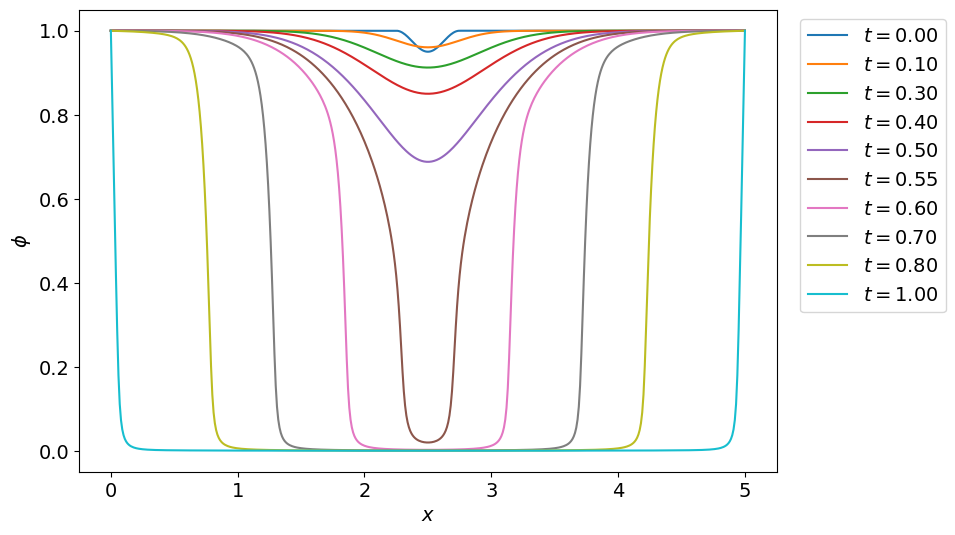
\includegraphics[width=\textwidth]{figures/typical_solution.png}
\end{figure}
\column{0.12\textwidth}
\hfill \\
\vspace{3.5cm}
\hspace{-2.5cm}
Из работы \cite{ponomarev_stability}. \\
\hspace{-2.5cm}
Узлов по измерениям: \\
\hspace{-2.5cm}
$N_x = 10^3$, $N_t = 10^5$
\end{columns}
\end{frame}


\begin{frame}{Цель работы}
\begin{itemize}
	\item Типичное поведение модели: долгий период медленных изменений, \\ затем стремительное развитие пробоя.
\end{itemize}
\begin{block}{Цель работы}
	Исследовать несколько подходов к адаптации расчетного шага по времени.
\end{block}
\end{frame}

%!TEX root = ../main.tex

\section{Методы адаптации}

\begin{frame}{Общий вид схемы с адаптивным шагом}
\begin{itemize}
	\item Вводится переменный шаг $\tau^k$:
	\[
		\phi_j^{k + 1} = \phi_j^k + m \tau^k \left( -F'(\phi_j^k) + \cfrac{\Gamma}{2} \diffhh{\phi} \right)
	\]
	\item Значение $\tau^k$ ограничено заранее выбранными $\tau_{min}$ и $\tau_{max}$:
	\[
		\tau^k = \max \left[ \tau_{min}, \min( \tau_{max}, \widetilde{\tau}^k) \right]
	\]
\end{itemize}
\end{frame}


\begin{frame}{Методы адаптации}
\vspace{-0.7cm}
\begin{block}{Методы адаптации}
	\begin{itemize}
		\item По фазовому полю:
		\[
			\widetilde{\tau}_1^k = \cfrac{tol_1}{\left\| \left[ \partt{\phi} \right]_h \right\|_C}
		\]
		\item По полной энергии:
		\[
			\widetilde{\tau}_2^k = \cfrac{tol_2}{\left| \left[ \cfrac{d \Pi}{dt} \right]_h \right|}
		\]
	\end{itemize}
\end{block}
Предложены в работах [?] и [?].
\end{frame}

{\nologo
\begin{frame}{Методы адаптации}
\vspace{-0.6cm}
\begin{itemize}
	\item Условие устойчивости схемы:
	\vspace{-0.3cm}

	\[
		\tau \leqslant \cfrac{1}{4m} \min \left( \cfrac{\delta^{5/3}}{|\nabla \Phi|^2 \epsilon_0}, \cfrac{h^2}{\Gamma} \right)
	\]
	\vspace{-0.3cm}
	\item Неравенство с первым аргументом $\min$ можно переписать в виде
	\[
		m \tau \max\limits_{\phi \in [0, 1]} |F''(\phi)| \leqslant 1
	\]
\end{itemize}
\vspace{-0.3cm}
\begin{block}{Адаптация по устойчивости}
	\[
		\widetilde{\tau}_3^k = \cfrac{tol_3}{m \cdot \max\limits_{j = 0}^N G(\phi_j^k)},
	\]
	где $G(\phi)$ мажорирует $|F''(\phi)|$
\end{block}
\end{frame}
}

%!TEX root = ../main.tex

\section{Вычислительный эксперимент}

\begin{frame}{Параметры модели}
\vspace{-1cm}
\begin{itemize}
	\item Параметры, отражающие реальный физический эксперимент:
\end{itemize}
\centering
\begin{tabular}{|l|c|l|}
	\hline
	Название & Переменная & Значение \\
	\hline
	электрическое напряжение		& $|\nabla \Phi|$	& $5.625 \cdot 10^6 \; \unitV / \unitm$							\\
	энергия роста канала			& $\Gamma$			& $8.118 \cdot 10^{-10} \; \unitJ / \unitm$						\\
	диэлектрическая проницаемость	& $\epsilon_0$		& $2.301 \cdot 10^{-11} \; \unitC^2 / (\unitJ \cdot \unitm)$	\\
	подвижность						& $m$				& $12 \; \unitm^3 / (\unitJ \cdot \units)$						\\
	\hline
	толщина границы					& $l$ 				& $1.5 \cdot 10^{-6} \; \unitm$									\\
	регуляризующий параметр 		& $\delta$			& $10^{-3}$														\\
	размер образца					& $L$				& $3.2 \cdot 10^{-5} \; \unitm$									\\
	продолжительность				& $T$				& $2 \cdot 10^{-3} \; \units$									\\
	шаг по пространству				& $h$				& $5 \cdot 10^{-7} \; \unitm$									\\
	минимальный шаг по времени		& $\tau_{min}$		& $10^{-10} \; \units$											\\
	максимальный шаг по времени		& $\tau_{max}$		& $\leqslant 6.42 \cdot 10^{-6} \; \units$						\\
	\hline
\end{tabular}
\end{frame}


\begin{frame}{Поведение системы}
\vspace{-0.4cm}
\begin{figure}
	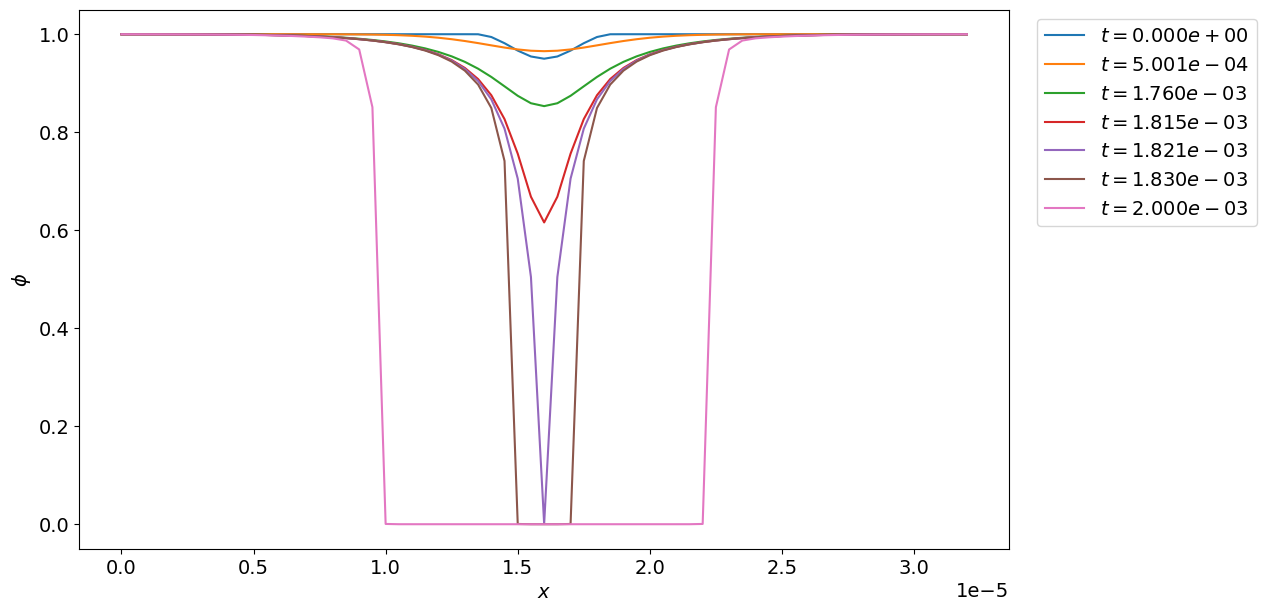
\includegraphics[width=0.87\textwidth]{figures/system_behaviour.png}
\end{figure}
\end{frame}


\begin{frame}{Результаты расчетов}
\centering
\begin{tabular}{|l|c|c|c|}
	\hline
	Тип адаптации & Ускорение (раз) & Отклонение по $\phi$ & Запаздывание \\
	\hline \hline
	по фазовому полю	& 800	& $3.64 \cdot 10^{-4}$	& $0.3\%$		\\
	по энергии			& 107	& $5.38 \cdot 10^{-4}$	& $0.36\%$		\\
	по устойчивости		& 1474	& $1.54 \cdot 10^{-2}$	& $0.71\%$		\\
	\hline \hline
	по фазовому полю	& 101	& $1.23 \cdot 10^{-5}$	& $0.004\%$		\\
	по энергии			& 101	& $3.27 \cdot 10^{-4}$	& $0.19\%$		\\
	по устойчивости		& 100	& $2.23 \cdot 10^{-5}$	& $0.0046\%$	\\
	\hline
\end{tabular}
\end{frame}

%!TEX root = ../main.tex

\section{Заключение}

Настоящая работа продолжает исследование, начатое в статье \cite{zipunova_higher_codimension}. Как было отмечено ее авторами, исследование это хотя и проводится для конкретной задачи, но, вероятно, затрагивает вопросы, содержащиеся в методе диффузной границы как таковом. Суть этих вопросов в том, позволяют ли уравнения среды с диффузной границей в своей <<классической>> редакции адекватно описывать включения, по своей природе являющиеся объектами высшей коразмерности. В качестве возможного ответа авторы работы \cite{zipunova_higher_codimension} предлагают определенного вида обобщение исходной модели.

Целью настоящей работы было численно исследовать упомянутое обобщение. В этом достигнуты определенные успехи. С помощью модификации метода конечных объемов преодолены трудности, связанные с необходимостью задавать граничные условия на множествах коразмерности 2 и 3 в трехмерном пространстве и с наличием у функции-решения  особенности в точках этих множеств. Указанный подход существенно не привязан к рассматриваемой модели -- в дальнейшем он может быть использован и в других задачах.

В некоторых случаях при построении разностной схемы возникали фундаментальные препятствия: оказывалось, что необходимых базисных функций попросту не существует. На основании этого выдвинута гипотеза, что в указанных случаях рассматриваемая дифференциальная задача поставлена некорректно и не имеет решения. Рассуждения вполне согласуется с теоретическими результатами работы \cite{zipunova_higher_codimension}. В будущем возможно строгое обоснование представленной гипотезы.


\begin{frame}{Литература}
\printbibliography
\end{frame}

\begin{frame}{}
\begin{center}
	\Large
	Спасибо за внимание!
\end{center}
\end{frame}

\end{document}